\documentclass{beamer}
\usepackage[utf8x]{inputenc}
\usepackage{pgfplots}
\usepackage{tikz}
\usetikzlibrary{positioning,shapes,shadows,arrows,chains}
\usepackage{mathtools,amsfonts,amssymb}
\usepackage{graphicx}
\usetheme{Singapore}
\setbeamertemplate{footline}[frame number]

\tikzset{
	cell/.style={
		rectangle split,
		rectangle split parts=2,
		rectangle split part fill={lightgray,cyan!25},
		draw
	}
}

\begin{document}

\title{Alignment in C}
\subtitle{Seminar "Effiziente Programmierung in C"}
\date{2014-01-09}
\author{Sven-Hendrik Haase}
\institute{Universität Hamburg, Fakultät für Informatik}

\begin{frame}
    \titlepage
\end{frame}
%It's basically like Tetris but with computer memory

\begin{frame}{Outline}
    \tableofcontents
\end{frame}

\section{Introduction}
\subsection{Memory addressing}
\begin{frame}{\insertsection}{\insertsubsection}
	\begin{itemize}
		\item Computers address memory in word sized chunks
		\item A word is a computer's natural unit for data
		\item Word size is defined by architecture
		\item 4 byte on 32-bit, 8 byte on 64-bit
		\item This means we can only address data at memory locations that are
			  multiples of 4 or 8 respectively
	\end{itemize}
	\pause
	\begin{center}
		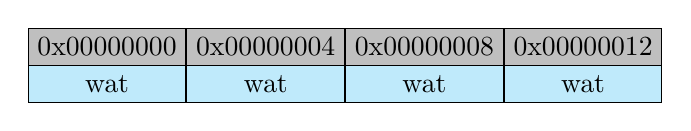
\begin{tikzpicture}[start chain, node distance=0, every on chain/.style=cell]
			\node [on chain] {0x00000000 \nodepart{two}wat};
			\node [on chain] {0x00000004 \nodepart{two}wat};
			\node [on chain] {0x00000008 \nodepart{two}wat};
			\node [on chain] {0x00000012 \nodepart{two}wat};
		\end{tikzpicture}
	\end{center}
\end{frame}

\subsection{Alignment 101}
\begin{frame}{\insertsection}{\insertsubsection}
	\begin{itemize}
		\item Assume a 32-bit architecture with a word size of 4
		\item 
	\end{itemize}
\end{frame}

\section{Data Structure Alignment}
\begin{frame}{Data Structure Alignment}
	More Stuff
\end{frame}

\section{Stack Alignment}
\begin{frame}{Stack Alignment}
	Even More Stuff
\end{frame}

\section{Summary}
\begin{frame}{Summary}
	Summary stuff
\end{frame}

\begin{frame}{Resources}
	stuff
\end{frame}

\end{document}
